\part{Planning}
\frame{\partpage}

\begin{frame}{Planning}
	\begin{itemize}
		\pause\item An \textbf{agent} in an \textbf{environment}
		\pause\item The environment has a \textbf{state}
		\pause\item The agent can perform \textbf{actions} to change the state
		\pause\item The agent wants to change the state so as to achieve a \textbf{goal}
		\pause\item Problem: find a sequence of actions that leads to the goal
	\end{itemize}
\end{frame}

\begin{frame}{STRIPS planning}
	\begin{itemize}
		\pause\item \textbf{St}anford \textbf{R}esearch \textbf{I}nstitute \textbf{P}roblem \textbf{S}olver
		\pause\item Describes the state of the environment by a set of \textbf{predicates} which are true
		\pause\item Models a problem as:
			\begin{itemize}
				\pause\item The \textbf{initial state} (a set of predicates which are true)
				\pause\item The \textbf{goal state} (a set of predicates, specifying whether each should be true or false)
				\pause\item The set of \textbf{actions}, each specifying:
					\begin{itemize}
						\pause\item Preconditions (a set of predicates which must be satisfied for this action to be possible) 
						\pause\item Postconditions (specifying what predicates are made true or false by this action)
					\end{itemize}
			\end{itemize}
	\end{itemize}
\end{frame}

\newcommand{\emptyy}{
\includegraphics[height=0.1\textheight]{empty}}
\newcommand{\monkey}{
\includegraphics[height=0.1\textheight]{monkey}}
\newcommand{\banana}{
\includegraphics[height=0.1\textheight]{banana}}
\newcommand{\boxbox}{
\includegraphics[height=0.1\textheight]{crate}}

\lstset{language={},
	basicstyle=\scriptsize\ttfamily
}

\begin{frame}[fragile]{STRIPS example}
	\begin{columns}
		\begin{column}{0.45\textwidth}
			\begin{tabular}{c|c|c}
				  $A'$  &   $B'$  &   $C'$  \\\hline
				\emptyy & \banana & \emptyy \\
				\emptyy & \emptyy & \emptyy \\
				\monkey & \emptyy & \boxbox \\\hline
				  $A$   &   $B$   &    $C$
			\end{tabular}
		\end{column}
		\begin{column}{0.5\textwidth}
			\pause Initial state:
			\begin{lstlisting}
At(A),
BoxAt(C),
BananasAt(B')
			\end{lstlisting}
			
			\vspace{2ex}
			
			\pause Goal:
			\begin{lstlisting}
HasBananas
			\end{lstlisting}
		\end{column}
	\end{columns}
\end{frame}

\begin{frame}[fragile]{STRIPS example --- Actions}
	\begin{columns}
		\begin{column}{0.4\textwidth}
			\begin{tabular}{c|c|c}
				  $A'$  &   $B'$  &   $C'$  \\\hline
				\emptyy & \banana & \emptyy \\
				\emptyy & \emptyy & \emptyy \\
				\monkey & \emptyy & \boxbox \\\hline
				  $A$   &   $B$   &    $C$
			\end{tabular}
		\end{column}
		\begin{column}{0.58\textwidth}
			\begin{lstlisting}
Move(x, y)
  Pre:  At(x)
  Post: !At(x), At(y)

ClimbUp(x)
  Pre:  At(x), BoxAt(x)
  Post: !At(x), At(x')

ClimbDown(x')
  Pre:  At(x'), BoxAt(x)
  Post: !At(x'), At(x)

PushBox(x, y)
  Pre:  At(x), BoxAt(x)
  Post: !At(x), At(y),
        !BoxAt(x), BoxAt(y)

TakeBananas(x)
  Pre:  At(x), BananasAt(x)
  Post: !BananasAt(x), HasBananas
			\end{lstlisting}
		\end{column}
	\end{columns}
\end{frame}

\begin{frame}[fragile]{STRIPS example --- Solution}
%	\begin{columns}
%		\begin{column}{0.4\textwidth}
	\begin{center}
			\begin{tabular}{c|c|c}
				  $A'$  &   $B'$  &   $C'$  \\\hline
				\emptyy & \banana & \emptyy \\
				\emptyy & \emptyy & \emptyy \\
				\monkey & \emptyy & \boxbox \\\hline
				  $A$   &   $B$   &    $C$
			\end{tabular}
	\end{center}
%		\end{column}
%		\begin{column}{0.58\textwidth}
%			State:
%			\begin{lstlisting}
%At(A),
%BoxAt(C),
%BananasAt(B')
%			\end{lstlisting}
%		\end{column}
%	\end{columns}
\end{frame}

\begin{frame}[fragile]{STRIPS example --- Solution}
%	\begin{columns}
%		\begin{column}{0.4\textwidth}
	\begin{center}
			\begin{tabular}{c|c|c}
				  $A'$  &   $B'$  &   $C'$  \\\hline
				\emptyy & \banana & \emptyy \\
				\emptyy & \emptyy & \emptyy \\
				\emptyy & \emptyy & \boxbox\monkey \\\hline
				  $A$   &   $B$   &    $C$
			\end{tabular}
	\end{center}
%		\end{column}
%		\begin{column}{0.58\textwidth}
%			Action:
%			\begin{lstlisting}
%Move(A, C)
%			\end{lstlisting}
%			\pause State:
%			\begin{lstlisting}
%At(C),
%BoxAt(C),
%BananasAt(B')
%			\end{lstlisting}
%		\end{column}
%	\end{columns}
\end{frame}

\begin{frame}[fragile]{STRIPS example --- Solution}
%	\begin{columns}
%		\begin{column}{0.4\textwidth}
	\begin{center}
			\begin{tabular}{c|c|c}
				  $A'$  &   $B'$  &   $C'$  \\\hline
				\emptyy & \banana & \emptyy \\
				\emptyy & \emptyy & \emptyy \\
				\emptyy & \boxbox\monkey & \emptyy \\\hline
				  $A$   &   $B$   &    $C$
			\end{tabular}
	\end{center}
%		\end{column}
%		\begin{column}{0.58\textwidth}
%			Action:
%			\begin{lstlisting}
%PushBox(C, B)
%			\end{lstlisting}
%			\pause State:
%			\begin{lstlisting}
%At(B),
%BoxAt(B),
%BananasAt(B')
%			\end{lstlisting}
%		\end{column}
%	\end{columns}
\end{frame}

\begin{frame}[fragile]{STRIPS example --- Solution}
%	\begin{columns}
%		\begin{column}{0.4\textwidth}
	\begin{center}
			\begin{tabular}{c|c|c}
				  $A'$  &   $B'$  &   $C'$  \\\hline
				\emptyy & \banana\monkey & \emptyy \\
				\emptyy & \boxbox & \emptyy \\\hline
				  $A$   &   $B$   &    $C$
			\end{tabular}
	\end{center}
%		\end{column}
%		\begin{column}{0.58\textwidth}
%			Action:
%			\begin{lstlisting}
%ClimbUp(B)
%			\end{lstlisting}
%			\pause State:
%			\begin{lstlisting}
%At(B'),
%BoxAt(B),
%BananasAt(B')
%			\end{lstlisting}
%		\end{column}
%	\end{columns}
\end{frame}

\begin{frame}[fragile]{STRIPS example --- Solution}
%	\begin{columns}
%		\begin{column}{0.4\textwidth}
	\begin{center}
			\begin{tabular}{c|c|c}
				  $A'$  &   $B'$  &   $C'$  \\\hline
				\emptyy & 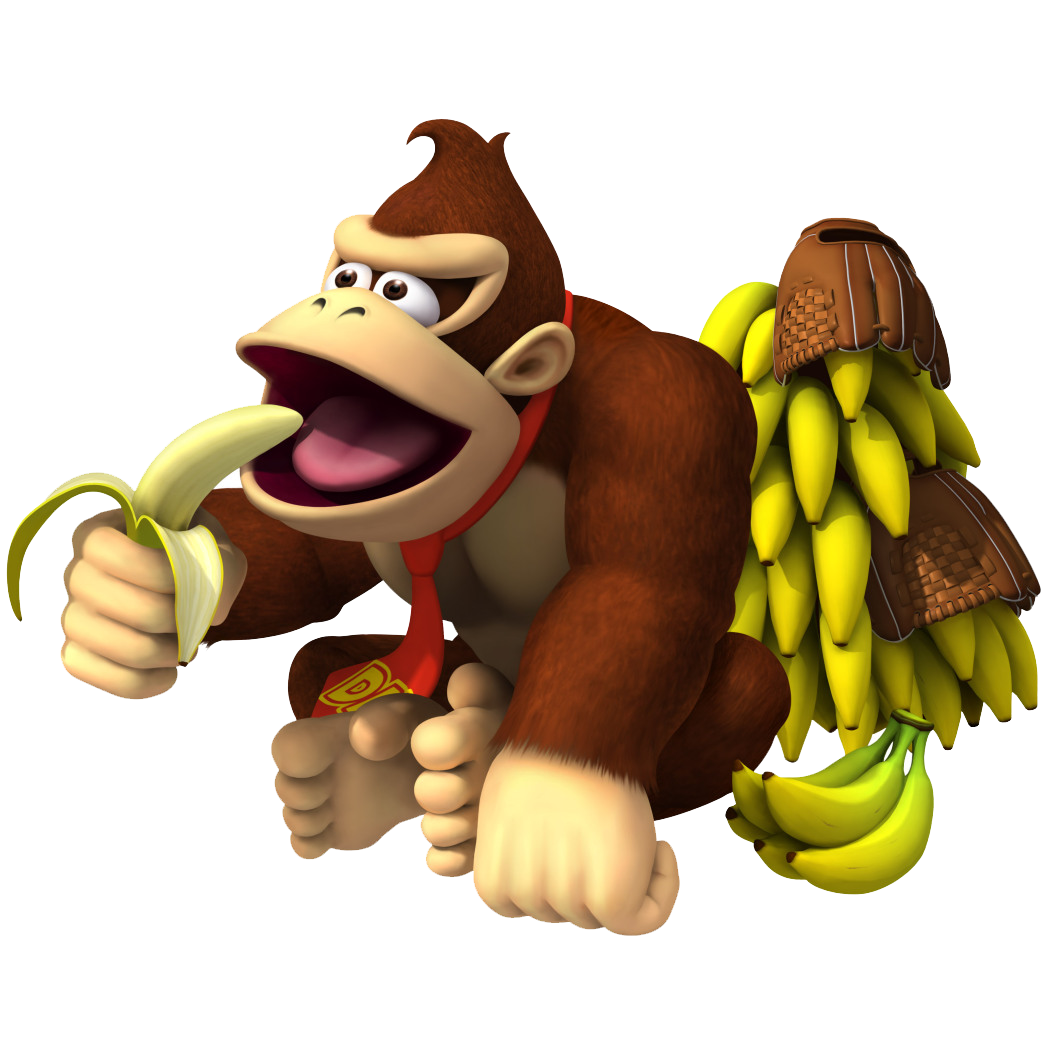
\includegraphics[height=0.2\textheight]{monkey_hasbananas} & \emptyy \\
				\emptyy & \boxbox & \emptyy \\\hline
				  $A$   &   $B$   &    $C$
			\end{tabular}
	\end{center}
%		\end{column}
%		\begin{column}{0.58\textwidth}
%			Action:
%			\begin{lstlisting}
%TakeBananas(B')
%			\end{lstlisting}
%			\pause State:
%			\begin{lstlisting}
%At(B'),
%BoxAt(B),
%HasBananas
%			\end{lstlisting}
%		\end{column}
%	\end{columns}
\end{frame}

\begin{frame}{Finding the solution}
	\begin{itemize}
		\pause\item For a given state, we can construct a list of all \textbf{valid actions}
			based on their \textbf{preconditions}
		\pause\item We can also find the \textbf{next state} resulting from each action
			based on their \textbf{postconditions}
		\pause\item We can construct a \textbf{state-action graph}
		\begin{itemize}
			\pause\item Nodes: environment states
			\pause\item Edges: actions
		\end{itemize}
		\pause\item We can then \textbf{search} this tree to find a goal state
	\end{itemize}
\end{frame}

\begin{frame}{Searching for the solution}
	\begin{itemize}
		\pause\item We have a \textbf{tree}, which is a type of \textbf{graph}
		\pause\item We have an \textbf{initial node} within this tree
		\pause\item Want to find a \textbf{sequence of edges} that leads to a \textbf{goal node}
		\pause\item Does this sound familiar?
		\pause\item Very similar to \textbf{pathfinding}, so can use the same algorithms (recall from COMP280 session 8)
		\begin{itemize}
			\pause\item Depth-first search
			\pause\item Breadth-first search
			\pause\item Dijkstra's algorithm
			\pause\item A$^*$ (if we have a suitable \textbf{heuristic})
		\end{itemize}
	\end{itemize}
\end{frame}
